%%%%%%%% ICML 2025 EXAMPLE LATEX SUBMISSION FILE %%%%%%%%%%%%%%%%%

\documentclass{article}
\usepackage{tikz}
\usepackage{tikz}
\usetikzlibrary{shapes.geometric, arrows, positioning}

\tikzstyle{layer} = [rectangle, rounded corners, minimum width=3.5cm, minimum height=1cm, text centered, draw=black, fill=blue!20]
\tikzstyle{arrow} = [thick,->,>=stealth]

% Recommended, but optional, packages for figures and better typesetting:
\usepackage{microtype}
\usepackage{graphicx}
\usepackage{subfigure}
\usepackage{booktabs} % for professional tables



% hyperref makes hyperlinks in the resulting PDF.
% If your build breaks (sometimes temporarily if a hyperlink spans a page)
% please comment out the following usepackage line and replace
% \usepackage{icml2025} with \usepackage[nohyperref]{icml2025} above.
\usepackage{hyperref}


% Attempt to make hyperref and algorithmic work together better:
\newcommand{\theHalgorithm}{\arabic{algorithm}}

% Use the following line for the initial blind version submitted for review:
% \usepackage{icml2025}

% If accepted, instead use the following line for the camera-ready submission:
\usepackage[accepted]{icml2025}

% For theorems and such
\usepackage{amsmath}
\usepackage{amssymb}
\usepackage{mathtools}
\usepackage{amsthm}

% if you use cleveref..
\usepackage[capitalize,noabbrev]{cleveref}

%%%%%%%%%%%%%%%%%%%%%%%%%%%%%%%%
% THEOREMS
%%%%%%%%%%%%%%%%%%%%%%%%%%%%%%%%
\theoremstyle{plain}
\newtheorem{theorem}{Theorem}[section]
\newtheorem{proposition}[theorem]{Proposition}
\newtheorem{lemma}[theorem]{Lemma}
\newtheorem{corollary}[theorem]{Corollary}
\theoremstyle{definition}
\newtheorem{definition}[theorem]{Definition}
\newtheorem{assumption}[theorem]{Assumption}
\theoremstyle{remark}
\newtheorem{remark}[theorem]{Remark}

% Todonotes is useful during development; simply uncomment the next line
%    and comment out the line below the next line to turn off comments
%\usepackage[disable,textsize=tiny]{todonotes}
\usepackage[textsize=tiny]{todonotes}


% The \icmltitle you define below is probably too long as a header.
% Therefore, a short form for the running title is supplied here:
\icmltitlerunning{Zero-Shot Forecasting and Neural Operators - Master Lab}

\begin{document}

\twocolumn[
\icmltitle{Zero-Shot Forecasting and Neural Operators \\ Master Lab
}

% It is OKAY to include author information, even for blind
% submissions: the style file will automatically remove it for you
% unless you've provided the [accepted] option to the icml2025
% package.

% List of affiliations: The first argument should be a (short)
% identifier you will use later to specify author affiliations
% Academic affiliations should list Department, University, City, Region, Country
% Industry affiliations should list Company, City, Region, Country

% You can specify symbols, otherwise they are numbered in order.
% Ideally, you should not use this facility. Affiliations will be numbered
% in order of appearance and this is the preferred way.

\begin{icmlauthorlist}
\icmlauthor{Arwin Sadaghiani}{yyy}
\icmlauthor{Jan Hardtke}{yyy}
\icmlauthor{Nadia Gharbi}{yyy}

\end{icmlauthorlist}

\icmlaffiliation{yyy}{Department of XXX, University of YYY, Location, Country}

\icmlcorrespondingauthor{Firstname1 Lastname1}{first1.last1@xxx.edu}
\icmlcorrespondingauthor{Firstname2 Lastname2}{first2.last2@www.uk}

% You may provide any keywords that you
% find helpful for describing your paper; these are used to populate
% the "keywords" metadata in the PDF but will not be shown in the document
\icmlkeywords{Machine Learning, ICML}

\vskip 0.3in
]

% this must go after the closing bracket ] following \twocolumn[ ...

% This command actually creates the footnote in the first column
% listing the affiliations and the copyright notice.
% The command takes one argument, which is text to display at the start of the footnote.
% The \icmlEqualContribution command is standard text for equal contribution.
% Remove it (just {}) if you do not need this facility.

%\printAffiliationsAndNotice{}  % leave blank if no need to mention equal contribution


\section{Introduction}

Time series modeling plays a vital role in fields such as climate science \cite{climate}, medicine \cite{medicine}, finance \cite{finance}, and retail \cite{retail}. The objective is to capture temporal patterns for predictions of future time horizons. However, real-world time series data are often sparse and noisy, requiring interpolation to create a smooth, continuous representation. This assumes the data stem from an underlying hidden function, which we can approximate for tasks like forecasting.

In this report, we propose a machine learning approach using neural operators for time series forecasting in a zero-shot learning setting.
Zero-shot learning enables models to generalize to new datasets, even beyond their training distribution, making it a promising method for building foundational models. 
As real-world data is often scarce, we generate multiple synthetic datasets by creating functions that capture trends and periodicity, combined with Gaussian noise to model observations of real-world phenomena.

The core idea of our method is to train a neural operator capable of mapping sparse time series observations into a smooth, continuous function space. This enables querying the predicted continuous function at arbitrary time points. The original concept is inspired by the FIM paper \cite{fim-l}, which leverages such neural operators for zero-shot imputation of observation gaps. Our approach extends this method by shifting the focus from imputing missing values to reconstructing a future time horizon based on observed past values.

The contributions of this work are as follows: (1) We create a synthetic dataset with 100K one-dimensional target functions sampled from a Gaussian Processes using multiple variants of kernels.

(2) Following the work of \cite{fim-l}, we utilize two models: FIM-$\ell$, based on the work of DeepONet \cite{Deeponet}, and FIM \cite{fim-l}. The first model, FIM-$\ell$, is responsible for learning local embeddings for localized windows of a given set of observations. These embeddings are then utilized by the second model, FIM, to predict the underlying function at future time horizons.

 (3) Finally, we aim to refine these architectures by experimenting with different variations of the architecture and training objectives. These modifications are then evaluated on both our synthetic validation datasets and a real-world dataset.

\section{Related Work}
Statistical methods, such as ARIMA, have a long-standing history in time series forecasting. ARIMA, which stands for Autoregressive (AR), Integrated (I), and Moving Average (MA), combines these three components to model stationary time series data—where the mean and variance of the underlying process remain constant over time.

The autoregressive (AR) component predicts future values as a linear combination of previously observed values. The integrated (I) component addresses non-stationarity by applying differencing operations (of order $d$) to stabilize the mean and variance of the time series. Stationarity, a key assumption of ARIMA, is achieved through transformations such as differencing or logarithmic scaling. Finally, the moving average (MA) component incorporates past forecast errors into predictions, rather than relying solely on observed values.

These components are combined into the full ARIMA model, which is expressed as:
\begin{equation}
y'_t = c + \phi_1 y'_{t-1} + \dots + \phi_p y'_{t-p} + \epsilon_t + \theta_1 \epsilon_{t-1} + \dots + \theta_q \epsilon_{t-q},
\end{equation}
where $y'_t$ represents the differenced time series, $\phi$ and $\theta$ are the model coefficients, and $\epsilon_t$ is the forecast error. This formulation allows ARIMA to effectively capture the structure of stationary time series data while accounting for both observed values and forecast errors.

Although ARIMA performs well on univariate and stationary datasets, it faces limitations with non-linear patterns and high-dimensional data \cite{stellwagen2013arima}. To address these challenges, deep learning approaches have gained increasing attention \cite{stellwagen2013arima}. One recent advance is TimesFM \cite{das2024decoderonlyfoundationmodeltimeseries}, a decoder-only foundation model designed for time series forecasting. Inspired by large language models, TimesFM is pre-trained on a diverse corpus of real-world and synthetic time series data, enabling it to capture complex temporal patterns across domains. It utilizes a decoder-style attention mechanism and input patching, similar to the approach used in vision transformers. TimesFM demonstrates strong zero-shot forecasting performance on both in-distribution and out-of-distribution (zero-shot) datasets, without requiring fine-tuning. Additionally, it is capable of handling varying forecasting horizons and time granularities.

Building on these advancements, this work investigates neural approaches, like TimesFM, to address challenges in time series forecasting.

%%%%%%%%%%%%%%%%%%%%%%%%%%%%%%%%%%% Report Start %%%%%%%%%%%%%%%%%%%%%%%%%%%%%%%%%%%%%%%%%%%%
%%%%%%%%%%%%%%%%%%%%%%%%%%%%%%%%%%%%%%%%%%%%%%%%%%%%%%%%%%%%%%%%%%%%%%%%%%%%%%%
\section{Problem Definition}
The goal of our project was to create a model which forecasts the future points of a time-series in a zero-shot manner. Concretely we want to build a model, that takes in $k$ previous windows of length $L$ of a time-series and then predicts the next $k+1$ window of length $L$. The model should also work in a zero-shot manner, meaning it should work without requiring any fine-tuning on the specific data it will be used on. To accomplish this we constructed a synthetic training dataset, built to cover a wide range of different time-series for the model to learn in order to facilitate the zero-shot use of the model. We also added artificial noise into our time-series data to make the model more robust and usable for real-world data. Our model consists  of two separate networks, one for encoding the $k$ windows and a second one for predicting the window $k+1$ from the encodings. 

\section{Methods}
In this section we will look at the two main architectures that our model is based on. We will first look at DeepONet~\cite{Deeponet}, which encodes our time-series windows and fits a function on the noisy time points, in Section \ref{sec:DeepONet} and afterwards at FIM~\cite{fim-l}, which predicts the future encoding, in Section \ref{sec:FIM_arwin}.

\subsection{DeepONet}\label{sec:DeepONet}
Deep operator network (DeepONet)\cite{Deeponet} is a neural network architecture designed to learn nonlinear operators more accurately and efficiently than standard fully-connected networks. DeepONet consists of two sub-networks, a branch net and a trunk net. The branch net takes in $m$ fixed values of the input function $f(\tau)$ and encodes them while the trunk net takes in the time point $t$ for the output function we want to predict and encodes it. Both networks return a $p$-dimensional encoding and to obtain the output function value at our time point $t$, the scalar product between both encodings is calculated.


\subsection{FIM}\label{sec:FIM_arwin}
FIM\cite{fim-l} is a model originally designed for the interpolation of time series displaying temporal missing patterns. Meaning we have our $k$ embeddings from $1, 2, ..., q-1, q+1, ..., k$ with the embedding $q$ missing. The task of FIM was then to predict the embedding for window $q$ from the other embeddings. In our work we used the core ideas of FIM but for forecasting the future embedding $k+1$. For this FIM takes in the embeddings $h_1, .., h_k$ along with local scale embeddings $s_1, .., s_k$. These scale embeddings are created by saving the normalization values, used to normalize the time-series data for each respective window, and feeding them through a MLP to obtain an embedding. Both embeddings then get concatenated and fed through a transformer and summary network to obtain the embedding $h_{k+1}$. With this embedding we can use the trunk net from DeepONet to obtain a function for future time points $t$.

\section{Synthetic Dataset}
\label{sec:dataset_arwin}
To train and test our models, we generated two synthetic datasets, each tailored to its respective model, consisting of time series.

For the DeepONet model, we constructed a dataset comprising \( 100{,}000 \) random one-dimensional target interpolation functions \( f(\tau) \), where \( \tau \in [0, 1] \). Each function is defined on a uniform grid of 128 points and sampled from a Gaussian Process (GP) with a mean function of \( 0 \) and a Radial Basis Function (RBF) kernel given by
\[
k(\tau, \tau') = \sigma^2 \exp\left(-\frac{\|\tau - \tau'\|^2}{2l^2}\right),
\]
where \( \sigma^2 \) is the variance of the Gaussian Process, determining the magnitude of variations in \( f(\tau) \), and \( l \) is the length scale, controlling the smoothness of the sampled functions.

The length scale is drawn randomly from a beta distribution and scaled by $0.1$ to increase the frequency of the sampled functions $f$ in our dataset.\\
Depending on whether we are creating a training or validation dataset, the values of \(\alpha\) and \(\beta\) for the beta distributions are uniform selected from either \([1.0, 2.0, 5.0]\) or \([0.5, 3.25, 7.8]\), respectively. The variance \(\sigma^2\) for the kernel is drawn uniformly from the interval \([0.5, 2]\).
We then sample random observation grid points \(\tau\) from our functions, which serve as inputs for our model. A random subset of points, between \(\text{min}=50\) and \(\text{max}=90\), is selected from the 128 grid points, and the remaining points are padded with \(0\)'s. Additionally, we create a binary mask for each observation grid to indicate which indices are observed versus unobserved. This mask is provided to the model along with the observed points.

Half of the observation points \(\tau\) are sampled regularly, while the other half are sampled irregularly in time. To account for noise in real-world applications, Gaussian noise \(\epsilon \sim \mathcal{N}(0, 0.1)\) with mean \(0\) is added to the observations after normalizing the data.

The normalization process involves applying z-scoring to the function values \(f(\tau)\) and min-max scaling to the time points \(\tau\). The normalized values are computed as follows:

\[
\hat{f}(\tau) = \frac{f(\tau) - \mu}{\sigma}, \quad \hat{\tau} = \frac{\tau - \tau^{\text{min}}}{\tau^{\text{max}} - \tau^{\text{min}}},
\]

where \(\mu\) and \(\sigma\) denote the mean and standard deviation of the function values \(f(\tau)\), and \(\tau^{\text{min}}\) and \(\tau^{\text{max}}\) represent the minimum and maximum values of the observation points \(\tau\). This approach ensures that the function values \(\hat{f}(\tau)\) are standardized, while the time points \(\hat{\tau}\) are scaled to the interval \([0, 1]\).
\\
For the FIM model, we created a dataset comprising \(100{,}000\) random one-dimensional target functions \(f(\tau)\) defined on the interval \([0, 1]\) and evaluated on a fine grid of 640 points. These functions were sampled from Gaussian Processes with a mean function of \(0\) and different kernels. The dataset distribution is composed as follows: periodic kernel \(k_p\) (30\%), locally periodic kernel \(k_{lp}\) (30\%), linear plus periodic kernel \(k_{lpp}\) (20\%), and linear times periodic kernel \(k_{ltp}\) (20\%).

The kernels are defined as:
\begin{align*}
    k_p(\tau, \tau') &= \sigma^2 \cdot \exp\left(-\frac{2\sin^2\left(\pi |\tau - \tau'| / p\right)}{l^2}\right), \\
    k_{lp}(\tau, \tau') &= k_p(\tau, \tau') \cdot \exp\left(-\frac{(\tau - \tau')^2}{2l^2}\right), \\
    k_{lpp}(\tau, \tau') &= k_p(\tau, \tau') + \sigma^2 \cdot (\tau \cdot \tau'^T), \\
    k_{ltp}(\tau, \tau') &= k_p(\tau, \tau') \cdot \sigma^2 \cdot (\tau \cdot \tau'^T).
\end{align*}

In addition to the length scale \(l\) and variance \(\sigma^2\), the kernels include a periodicity parameter \(p\). The length scale and periodicity are sampled from beta distributions. The parameters for these beta distributions are drawn either from \([1.0, 2.0, 5.0]\) for the training dataset or \([1, 1, 1]\) for the validation dataset.

The variance is drawn in the same manner as for the DeepONet dataset. We again sample random observation grid points \(\tau\) from our functions, which serve as inputs for our model. We divide the observations into \(K=5\) windows, where the first 4 windows serve as the context, and the \(K\)-th window is used as the prediction ground truth.

The first \(4\) windows are constructed in the same manner as for the DeepONet dataset, except that the standard deviation of the added noise is now drawn from \(\mathcal{N}(0, 0.025)\). One important detail is that, before normalizing each \(128\)-point window in the same way as for the DeepONet dataset, we first normalize the entire function by applying z-scoring to the function values and min-max scaling to \(\tau\).

Inspired by \cite{fim-l}, we save the local statistics of each window $l\leq K$ into a scales array \(s_l\), defined as:
\[
\begin{aligned}
s_l = [&\mu, \sigma, \max_{\tau} f(\tau) - \min_{\tau} f(\tau), \\
       &f(\tau^{\text{first}}), f(\tau^{\text{last}}), 
        f(\tau^{\text{last}}) - f(\tau^{\text{first}}), \\
       &\tau^{\text{first}}, \tau^{\text{last}}, 
        \tau^{\text{last}} - \tau^{\text{first}}].
\end{aligned}
\]


where \(\tau\) represents the sampled observations, and \(f\) denotes the noisy function values.



\section{Model architecture}
Next, we proceed with a detailed description of the architectures for both the FIM-l and FIM models. The FIM-l model serves as an operator, aiming to learn the underlying function from noisy samples, while the FIM model is designed as a forecasting framework. Our description closely follows the original implementations of both architectures, as outlined in the FIM paper \cite{fim-l}.

\subsection{FIM-$\ell$}\label{sec:FIM-l}
The primary aim of the FIM-$\ell$ model is to learn the underlying function $f(\tau)$ that has been augmented by noise to generate the observed time series $(y_i, \tau_i)$. The model should allow querying interpolated values of the underlying function $f(\tau)$ at arbitrary time points, including those not present in the observed data.
We can therefore think of FIM-$\ell$ as a learned \emph{neural interpolation operator} that maps the observed data into a continuous function space. To achieve this, we will leverage the ideas and architecture proposed by DeepONet \cite{Deeponet}.
Given our noisy input sequence \((y_1, \tau_1), \ldots, (y_l, \tau_l)\), with observation values \(y_i \in \mathbb{R}\) and ordered observation times \(\tau_i \in \mathbb{R}^+\), as well as query points \(t_i\), we define two feedforward neural network (FFN) embedding networks, \(\phi^{\theta}_0\) and \(\phi^{\theta}_1\), to transform both the observed values and time points into an embedded representation:
\[
    \hat{y_i} = \phi^{\theta}_0(y_i), \quad
    \hat{t_i} = \phi^{\theta}_1(t_i).
\]
We then proceed by concatenating both components to obtain the individual observation embeddings:
\[
    \mathbf{y^{\theta}_i} = \text{Concat}(\hat{y_i}, \hat{t_i}).
\]
Following the work of DeepONet, we define a \emph{branch net}-equivalent network consisting of a transformer-encoder network \cite{vaswani2023attentionneed}, denoted as $\psi^{\theta}_0$, and a multilayer perceptron (MLP), denoted as $\phi^{\theta}_3$. Together, these form
\[
    \mathbf{u^{\theta}} = \phi^{\theta}_3\big(\psi^{\theta}_0(\mathbf{y^{\theta}_1}, \dots, \mathbf{y^{\theta}_l})\big).
\]
Finally, to generate a sequence-length-agnostic embedding, we take \(\mathbf{u}^{\theta}\) from the branch network and feed it into a Multi-Head Attention \cite{} summary block $\lambda^{\theta}_0$, where \(\mathbf{u}^{\theta}\) serves as the \emph{keys} and \emph{values}, and a \emph{learnable} vector \(q_{\theta^*}\) is used as the \emph{query}. The attention calculation is defined as 

\[
\mathbf{h^{\theta}} = \text{softmax}\left(\frac{q_{\theta^*} K^\top}{\sqrt{d_k}}\right) V = \lambda^{\theta}_0(\mathbf{u}^{\theta}),
\]
where \(K = \mathbf{u}^{\theta}\) are the keys, \(V = \mathbf{u}^{\theta}\) are the values, and \(d_k\) is the dimensionality of the keys.\\
Next, we define our \emph{trunk net}-equivalent network. We begin by introducing a separate embedding network, $\phi^{\theta}_4$, for the query points $t$. Additionally, we define another MLP, $\phi^{\theta}_5$. The final trunk net output, $\mathbf{t}^{\theta}$, is then obtained as
\[
    \mathbf{t}^{\theta} = (\phi^{\theta}_5 \circ \phi^{\theta}_4)(t).
\]
To finally obtain the interpolated values of the learned underlying function at the query points $t$, we define a final MLP, $\phi^{\theta}_7$, such that
\[
    \mathbf{y}(t) = \phi^{\theta}_7\big(\text{Concat}(\mathbf{h}^{\theta}, \mathbf{t}^{\theta})\big),
\]
where $\mathbf{y}(t)$ represents the learned underlying function given our noisy observation values.

\subsection{FIM}\label{sec:FIM}
We now proceed by utilizing the learned representations \(\mathbf{h}^{\theta}\) of each local function window to predict the values of the time series at arbitrary points within the next, previously unseen window.
Starting from the beginning, we receive a noisy time sequence \((y_1, \tau_1), \ldots, (y_l, \tau_l)\). 
We then split these values into \(K=5\) windows, such that for window \(S_j\), we have
\[
S_{ji} = (y_{\alpha + i}, \tau_{\alpha + i}), \quad \alpha = \sum_{l=1}^{j-1}w_l,
\]
where \(w_l\) is the number of observations in window \(l \leq K-1\).
Additionally, for each of these windows, we construct their local scale characteristics \(s_l \in \mathbb{R}^9\) \ref{sec:dataset_arwin}, which are fed into an embedding layer \(\sigma^{\omega}_0\), defined as
\[
\hat{s_l} = \sigma^{\omega}_0(s_l).
\]
We then pass each window of observations into the pretrained embedding layers of the FIM-\(\ell\) model. Specifically, we define:
\[
    \mathbf{y}^j_i = \text{Concat}\big(\phi^{\theta}_0((S_{ji})_1), \phi^{\theta}_1((S_{ji})_2)\big), \quad \text j \leq K-1, i \leq w_j.
\]
We proceed by passing these \(\mathbf{y}^j\) into the branch network of the FIM-\(\ell\), resulting in
\[
    \mathbf{h}_j = (\lambda^{\theta}_0 \circ \phi^{\theta}_3 \circ \psi^{\theta}_0)\big(\mathbf{y}^{j}_1, \dots, \mathbf{y}^{j}_{w_j}\big).
\]
After extracting the local embeddings for each of the \(K-1\) windows, we proceed to reconstruct the \(K\)-th window. To achieve this, we first concatenate each local-scale embedding \(\hat{s}_j\) with the observation embeddings and feed them into a Transformer encoder block \(\psi^{\omega}_1\). This is again followed by an attention-based summary network \(\lambda^{\omega}_1\), which generates the final embedding for the \(K\)-th window
\[
    \mathbf{h}^{*}_K = (\eta^{\omega}_0 \circ \lambda^{\omega}_1 \circ \psi^{\omega}_1)\Big(( \mathbf{h}_1, \hat{s}_1), \ldots, \eta^{\omega}_0( \mathbf{h}_{K-1}, \hat{s}_{K-1})\Big).
\]
Due to the concatenation of the observation and scale embeddings, the feature dimension is now doubled compared to the original embedding size. However, the frozen projection network of FIM-\(\ell\) expects inputs in the original embedding dimension. To address this, we utilize an extractor network \(\eta^{\sigma}_0\), which transforms the output of the summary network $\lambda^{\omega}_1$ back to the dimension expected by the FIM-\(\ell\) projection layer.

To generate the final predictions for the \(K\)-th window, we utilize the embedding and trunk networks of the pretrained FIM-\(\ell\) to predict the function values at the query points \(t\). This is expressed as
\[
    \mathbf{y}(t) = \phi^{\theta}_7\big(\text{Concat}(\mathbf{h}^*_K, (\phi^{\theta}_5 \circ \phi^{\theta}_4)(t))\big).
\]
\section{Model Training}
In this section, we provide the necessary information to ensure the reproducibility of our work. Specifically, we outline the detailed structure of the aforementioned MLPs and discuss all relevant hyperparameters for both the model and the optimization algorithms.
\subsection{FIM-$\ell$ Training}\label{sec:FIM-l}
The implementation of our previously defined FIM-$\ell$ architecture is described in 
\ref{tab:architecture}. Here, we use \(d_{\text{model}}\) to denote the embedding dimension. In our setting, we set \(d_{\text{model}} = 256\) and \(n_{\text{heads}} = 4\). Since \emph{LeakyReLU} is shift-invariant, the bias term in the linear layer can be omitted if it is followed by a \emph{LayerNorm}, as the \emph{LayerNorm} neutralizes any bias introduced by the preceding layer.
We train the model with a batch size of 128, using the \emph{AdamW} optimizer with the following hyperparameters: \(\beta\)-values \((\beta_1, \beta_2) = (0.9, 0.999)\), \(\epsilon = 10^{-8}\), and a weight decay of \(0.01\). The training is performed for 20 epochs, which took approximately one hour.
Additionally, we employ an \emph{Inverse Square Root Learning Rate} (\emph{InverseSquareRootLR})\cite{??} scheduling strategy, 
with 100 warm-up steps, an initial learning rate of \(10^{-4}\), and a minimum learning rate of \(10^{-5}\).\\
To save memory and computational resources, we utilize the PyTorch \emph{Automatic Mixed Precision} package, which trains the model in mixed precision. Specifically, it selects half-precision data types (\emph{bfloat16} in our case) for operations it deems suitable. This approach enables the model to leverage the highly optimized NVIDIA Tensor Cores, maximizing performance during matrix operations.\\
For our loss computations, we use the standard \emph{Mean Squared Error} (MSE) between the predicted outputs of the model and the precomputed ground truth. Before performing the optimizer update step, we apply gradient clipping to ensure that the gradient norm does not exceed the length of a unit vector. This stabilizes training by limiting the size of each gradient step during optimization.\\
We then provide the model with the noisy observation sequence, observation time points, query points, and the branch mask. The branch mask is then utilized by both the Transformer encoder \(\psi^{\theta}_0\) and the summary network \(\lambda^{\theta}_0\) as the padding mask.



\begin{table}[h!]
    \centering
    \label{tab:architecture}
    \renewcommand{\arraystretch}{1.2} % Increase row height for readability
    \begin{tabular}{p{0.5\columnwidth} p{0.5\columnwidth}}
    \toprule
    \textbf{Component}               & \textbf{Details} \\ \midrule
    \textbf{Branch Embedding $\phi^{\theta}_0$}    & Linear(1, $d_\text{model}$) \\ \midrule
    \textbf{Branch Embedding $\phi^{\theta}_1$}    & Linear(1, $d_\text{model}$) \\ \midrule
    \textbf{Trunk Embedding $\phi^{\theta}_4$}         & Linear(1, $d_\text{model}$) \\ \midrule
    \textbf{Branch Encoder Input}    & Concatenate embeddings of $y$ and $t$ \\ \midrule
    \textbf{Branch Encoder $\psi^{\theta}_0$}          & Transformer Encoder (6 layers, $2d_\text{model}$, $n_\text{heads}$) \\ \midrule
    \textbf{Branch MLP $\phi^{\theta}_3$}              & Linear($2d_\text{model} \to d_\text{model}$), LeakyReLU, LayerNorm \\ \midrule
    \textbf{Learnable Query}         & Parameter tensor of shape (1, $d_\text{model}$) \\ \midrule
    \textbf{Branch Attention $\lambda^{\theta}_0$}        & Multihead Attention ($d_\text{model}$, heads=1) \\ \midrule
    \textbf{Trunk MLP $\phi^{\theta}_5$}               & 4x Linear($d_\text{model} \to d_\text{model}$), LeakyReLU, LayerNorm \\ \midrule
    \textbf{Combine Outputs}         & Concatenate outputs of Branch Attention and Trunk MLP \\ \midrule
    \textbf{Final Projection $\phi^{\theta}_7$}        & 5x Linear ($2d_\text{model} \to 1$), LeakyReLU, LayerNorm \\ 
    \bottomrule
    \end{tabular}
    \caption{FIM-$\ell$ architecture implementation}
    \end{table}
    

\subsection{FIM Training}\label{sec:FIM}
The implementation of the FIM network that we defined is detailed in Table~\ref{tab:architecture_megatron}. 
We set \(d_\text{model} = 256\) and \(n_\text{heads} = 8\). Regarding the optimizer and learning rate strategy, 
we use the same settings as described previously, along with automatic mixed precision training. 
The loss function remains the \emph{Mean Squared Error} (MSE), and the gradients are clipped to ensure their 
norm does not exceed the length of a unit vector.
We again provide the model with the noisy observation sequence, observation time points, query points, and the branch mask. However, instead of treating a single window as one data point, each example now comprises all local windows of the global function. We then continue training for 70 epochs, which takes approximately 4 hours. All model training was conducted on an NVIDIA RTX 3070 GPU, equipped with 8GB of GDDR6 VRAM.


\begin{table}[h!]
    \centering
    \label{tab:architecture_megatron}
    \renewcommand{\arraystretch}{1.2} % Increase row height for readability
    \begin{tabular}{p{0.45\columnwidth} p{0.5\columnwidth}}
    \toprule
    \textbf{Component}               & \textbf{Details} \\ \midrule
    \textbf{Pretrained FIM-$\ell$}   & $n_\text{heads-fim-$\ell$}$, $d_\text{model}$ (Frozen) \\ \midrule
    \textbf{Local Scale Embedding $\sigma^{\omega}_0$}   & Linear(9, $d_\text{model}$) \\ \midrule
    
    \textbf{Combine Outputs}         & Concatenate outputs of Pretrained FIM-$\ell$ and Local Scale Embedding \\ \midrule
    \textbf{Transformer Encoder $\psi^{\omega}_1$}     & 8 layers, $2d_\text{model}$, $n_\text{heads}$ \\ \midrule
    
    
    \textbf{Learnable Query}         & Parameter tensor of shape (1, $2d_\text{model}$)\\ \midrule
    \textbf{Summary Attention  $\lambda^{\omega}_1$}       & Multihead Attention ($2d_\text{model}$, $n_\text{heads}$) \\ \midrule
    
    \textbf{Extractor Network $\eta^{\omega}_0$} & 4x Linear ($2d_\text{model} \to d_\text{model}$), LeakyReLU, LayerNorm \\ \midrule
    
    \textbf{Trunk Embedding $\phi^{\theta}_4$}         & Reused from FIM-$\ell$ (Frozen)\\ \midrule
    \textbf{Trunk MLP $\phi^{\theta}_5$}           & Reused from FIM-$\ell$ (Frozen) \\ \midrule
    \textbf{Combine Outputs}         & Concatenate outputs of Trunk Network and Summary Network \\ \midrule
    \textbf{Final Projection $\phi^{\theta}_7$}        & Reused from FIM-$\ell$ (Frozen): \\ 
                                      & \quad 5x Linear ($2d_\text{model} \to 1$), LeakyReLU, LayerNorm \\ 
    \bottomrule
    \end{tabular}
    \caption{FIM Architecture Overview}

    \end{table}
    

\section{Experiments}
In this section, we discuss additional experiments conducted on the model's architecture and the construction of the loss function to achieve higher prediction accuracy. The impact of each of these approaches will be presented later in Section~\ref{sec:results}.

\subsection{Learned Positional Encoding for FIM-$\ell$ Embeddings}
In this approach, we hypothesize that the model may benefit from additional positional encoding for the attention-based summary network \(\lambda^{\omega}_1\). We define

\[
    \mathbf{p} =  \psi^{\omega}_1\Big(( \mathbf{h}_1, \hat{s}_1), \ldots, \eta^{\omega}_0( \mathbf{h}_{K-1}, \hat{s}_{K-1})\Big), \quad \mathbf{p} \in \mathbb{R}^{(K-1) \times d_{\text{model}}}.
\]

as the output from the FIM transformer encoder network. In our standard implementation, \(\mathbf{p}\) is passed to the summary attention network \(\lambda^{\omega}_1\), which, by default, lacks a sense of order among these embeddings, aside from the local scale statistics of each window. We hypothesize that providing positional information may help this layer better identify the order of embeddings, enabling more informed predictions of the \(K\)-th embedding.\\
To address this, we introduce an additional parameter vector \(\mathbf{z} \in \mathbb{R}^{(K-1) \times d_{\text{model}}}\), which serves as a learnable positional encoding. We add \(\mathbf{z}\) elementwise to \(\mathbf{p}\) before passing the result to \(\lambda^{\omega}_1\), as follows

\[
    \mathbf{h}^*_K = (\eta^{\omega}_0 \circ \lambda^{\omega}_1) \Big(\mathbf{p} + \mathbf{z} \Big).
\]



\subsection{Similarity loss between FIM-$\ell$ ground truth and predicted embeddings.}
Another strategy is the usage of the ground truth $\mathbf{h}_K$ for enabling more accurate predictions. The idea is to align the predicted $\mathbf{h}^*_K$ and the actual ground truth $\mathbf{h}_K$ such that they are as close as possible to each other. We can do this by adding an additional term to the model's loss function, which incentivizes it to form predictions $\mathbf{h}^*_K$ that are close to the FIM-$\ell$ predicted $\mathbf{h}_K$. A suitable metric for this is the \emph{cosine similarity}, defined as
\[
\text{CosSim}(\mathbf{a}, \mathbf{b}) = \frac{\mathbf{a}^T \mathbf{b}}{\|\mathbf{a}\| \|\mathbf{b}\|}, \quad \mathbf{a}, \mathbf{b} \in \mathbb{R}^n.
\]
\[
\forall \mathbf{a}, \mathbf{b} \in \mathbb{R}^n \setminus \{\mathbf{0}\}, \quad \text{CosSim}(\mathbf{a}, \mathbf{b}) \in [-1, 1].
\]


Geometrically, the \emph{cosine similarity} represents the cosine of the angle between two vectors. Specifically, $\text{CosSim}(\mathbf{a}, \mathbf{b}) = 0$ indicates orthogonality, while $\text{CosSim}(\mathbf{a}, \mathbf{b}) = 1$ and $\text{CosSim}(\mathbf{a}, \mathbf{b}) = -1$ correspond to vectors pointing in the same and opposite directions, respectively.\\
To give the network a better chance of transforming $\mathbf{h}^*_K$, we introduce an additional 4-layer MLP called $\lambda_2^{\omega}$. We then calculate the cosine similarity (CosSim) between the output of $\lambda_2^{\omega}$ and $\mathbf{h}_K$.\\
We now define our new loss function $\mathcal{L}(y, \hat{y}, \mathbf{h}^*_K, \mathbf{h}_K)$, which incorporates both prediction accuracy and alignment between the predicted and ground-truth representations. The loss function is given by
\[
\begin{aligned}
\mathcal{L}(y,\hat{y},\mathbf{h}^*_K,\mathbf{h}_K) &= 
\frac{1}{n}\sum_{i=1}^{n}(y_i - \hat{y}_i)^2   \\
&+ \beta \cdot |\text{CosSim}(\lambda_2^{\omega}(\mathbf{h}^*_K),\mathbf{h}_K) - 1|.
\end{aligned}
\]


where $y$ denotes the ground truth values of the target variable, and $\hat{y}$ represents the corresponding predicted values by the model. We choose $\beta = 0.2$ to ensure that the optimization does not focus too aggressively on aligning $\mathbf{h}^*_K$ and $\mathbf{h}_K$.






\section{Results}
\label{sec:results}

We will now discuss our findings regarding both the baseline architecture and the performance of our additional experiments. For evaluation, we utilize both our validation set and the \emph{ETTh1} dataset, which comprises real-world time series data from multiple domains.
\subsection{Findings on Validation Set}
On our validation set, we evaluate the performance of our models with the 
$\emph{Mean Absolute Error}$ (MAE) defined as
\[
\text{MAE}(y,\hat{y}) = \frac{1}{n}\sum_{1}^{n}|y_i-\hat{y}_i|.
\]
In Table~\ref{tab:evaluation_results}, we present the results on our validation set for multiple instances of our model. We abbreviate our Standard model with the capital letter S, as well as PE for positional encoding and CSL for cosine-similarity loss. Unfortunately, as shown in the table, neither the addition of positional encoding to the FIM-$\ell$ embeddings in the summary network nor the introduction of the cosine loss yielded any significant benefit. However, we observed a slightly lower training loss for the PE variant.

\begin{figure}[h!]
    \centering
    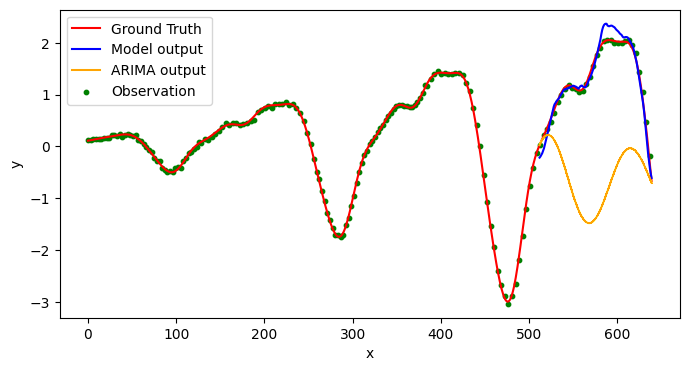
\includegraphics[width=\linewidth]{assets/validation1.png}
    \caption{Your caption here.}
    \label{fig:validation1}
\end{figure}
Looking at the plots of the predictions generated by our model on the validation set, we observed that the model performs well on data with high periodicity (see Figure~\ref{fig:validation1}). Since the functions and the parameters for the Gaussian process are sampled randomly, it is possible to encounter functions with less clear patterns (see Figure~\ref{fig:validation2}). These functions pose a challenge for the model, as it cannot anticipate their behavior in advance. This results in the model learning the average course of such functions. We postulate that this behavior negatively impacts the model's performance on functions where distinct patterns are present. It's therefore crucial to have checks in place to ensure that the model is only trained on data that exhibits clear patterns or aligns with the desired characteristics of the target task. This may help prevent the model from overfitting to noise or learning irrelevant trends.

 
\begin{figure}[h!]
    \centering
    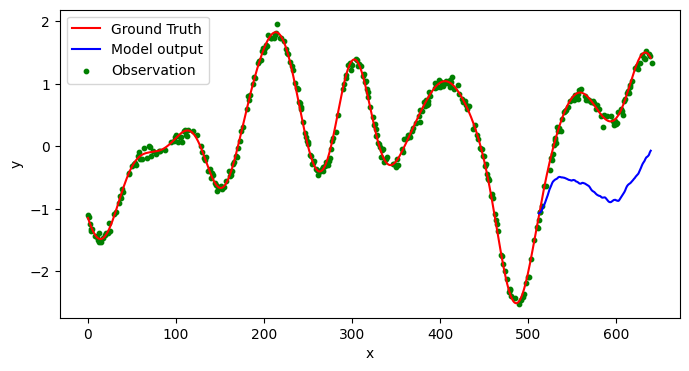
\includegraphics[width=\linewidth]{assets/validation2.png}
    \caption{Your caption here.}
    \label{fig:validation2}
\end{figure}

\subsection{Findings on ETTh1}
ETTh1 is a time series dataset containing data from various domains, such as oil temperature and electrical charge. We evaluate our model with a time horizon of 96, which corresponds to capturing 480 data points. These are split into $K=5$ windows, with the task being to predict the 5th window. 
The five windows are then shifted by one to the right and evaluated again.
The same procedure is applied for the time horizon of 192.
\begin{table}[h!]
    \centering
    \begin{tabular}{|c|c|c|c|c|}
    \hline
    \textbf{} & S & PE & PE + CSL & TimesFM \\ \hline 
    Validation   & 0.576             & 0.579             & 0.585             & -       \\ \hline
    ETTh1 - 96   & 0.966             & 0.968            & 0.928      &0.43*             \\ \hline
    ETTh1 - 192  & 1.0904            & 1.089            & 1.043            & 0.43*                     \\ \hline

\end{tabular}
    \caption{MAE results for three model variants and TimesFM on two datasets.\\
    \textit{*} TimesFM \cite{das2024decoderonlyfoundationmodeltimeseries} only reports the average score over both time horizons. Additionally, they use only 4 datasets from ETTh1, which they do not disclose.
    }
    \label{tab:evaluation_results}
\end{table}
We evaluate our different model variants on the entire ETTh1 dataset in a zero-shot manner, meaning that we evaluate on all sub-datasets contained within ETTh1 and calculate the average performance.
Additionally, we compare our model to the one proposed by TimesFM \cite{das2024decoderonlyfoundationmodeltimeseries}, using their accuracy score as a benchmark.
As shown in Table~\ref{tab:evaluation_results}, positional encoding does not appear to offer a significant benefit over the standard model. However, the PE + CSL approach provides slightly better performance. We also observe that the zero-shot performance of TimesFM on ETTh1-96 is much better than that of our current model. It is important to note, however, that TimesFM has been trained on a variety of data, both real-world and synthetic, and is approximately an order of magnitude larger in terms of parameter count.
We observe the same ordering of models for a horizon window of 192, where the PE + CSL version performs slightly better than the vanilla and PE versions.

\begin{figure}[h!]
    \centering
    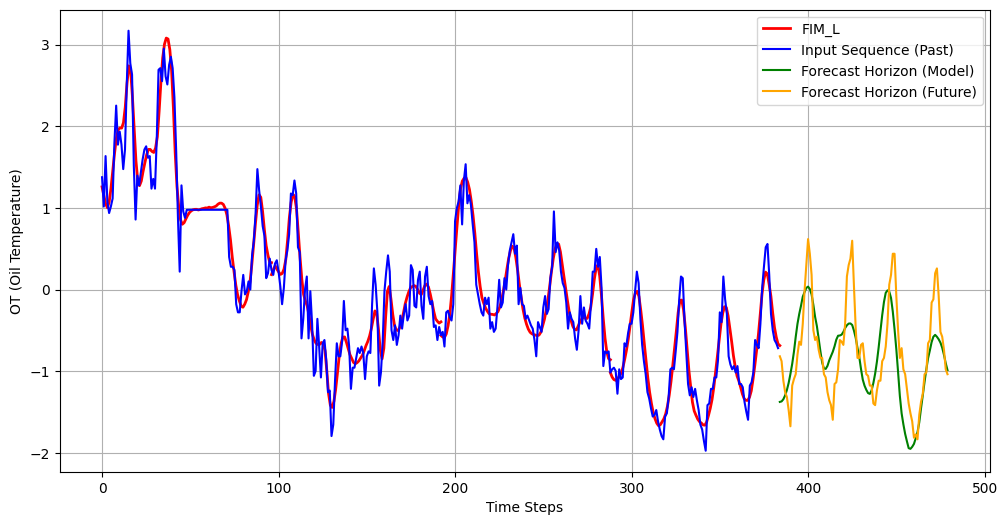
\includegraphics[width=\linewidth]{assets/etth128-success.png}
    \caption{Example of good performance on the oil temperature dataset with $\text{horizon}=96$, using the PE + CSL model version.
    }
    \label{fig:etth96-success}
\end{figure}
Finally, we present two examples from the ETTh1 dataset using our model to showcase both well-performing and poorly-performing cases. In Figure~\ref{fig:etth96-success}, the model successfully predicts the horizon, as the data follows a very predictable pattern. However, in Figure~\ref{fig:etth96-fail}, we observe that the model struggles to accurately predict the horizon probably due to the lack of a very clear pattern in the data.


\begin{figure}[h!]
    \centering
    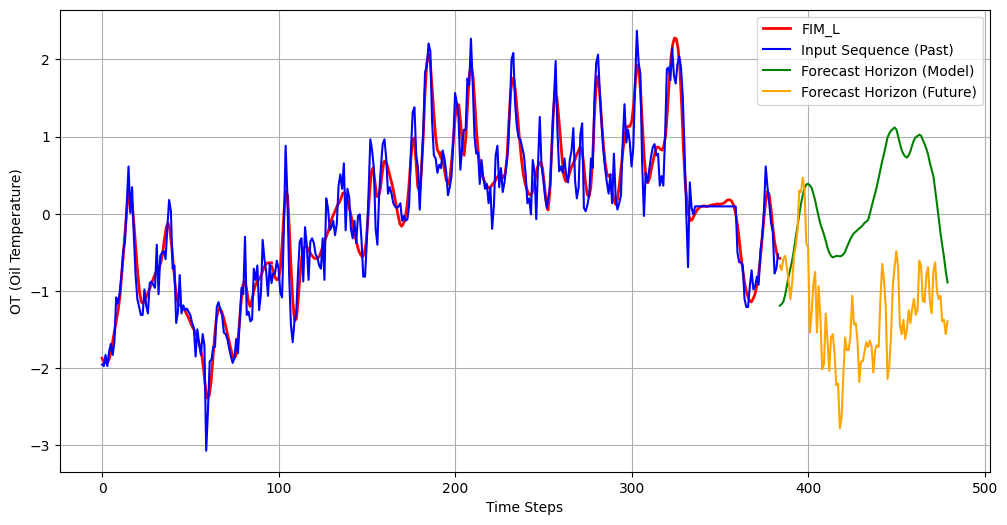
\includegraphics[width=\linewidth]{assets/etth128-fail.png}
    \caption{Example of bad performance on the oil temperature dataset with $\text{horizon}=96$, using the PE + CSL model version.
    }\label{fig:etth96-fail}
\end{figure}
This suggests that our networks would likely benefit significantly from training on more diverse and real-world datasets, allowing them to learn patterns that are more subtle than those generated by a Gaussian process with a periodic kernel.

\section{Conclusion}
In this work, we presented a novel approach for zero-shot forecasting by integrating the concepts of DeepONet and the FIM architecture to predict future horizons in time series data. To facilitate effective training, we constructed a synthetic dataset comprising randomly sampled periodic functions augmented with normally distributed noise.

To advance our architecture further, we experimented with several modifications, including the addition of positional encoding for local function embeddings and the introduction of an auxiliary loss function aimed at aligning the predicted embeddings of future horizons with their corresponding ground truth embeddings. 

We evaluated our approaches on both a validation set and the \emph{ETTh1} dataset. While the incorporation of positional encoding did not yield a significant performance improvement, the cosine similarity loss variant demonstrated a modest enhancement in predictive accuracy.

Our findings highlight the importance of carefully constructing datasets that exhibit genuine patterns to prevent the model from overfitting to noise. Additionally, integrating real-world datasets into the training process, as done by TimesFM, is essential for enhancing the model's applicability and performance in practical scenarios. 






\bibliography{example_paper}
\bibliographystyle{icml2025}


%%%%%%%%%%%%%%%%%%%%%%%%%%%%%%%%%%%%%%%%%%%%%%%%%%%%%%%%%%%%%%%%%%%%%%%%%%%%%%%
%%%%%%%%%%%%%%%%%%%%%%%%%%%%%%%%%%%%%%%%%%%%%%%%%%%%%%%%%%%%%%%%%%%%%%%%%%%%%%%
% APPENDIX
%%%%%%%%%%%%%%%%%%%%%%%%%%%%%%%%%%%%%%%%%%%%%%%%%%%%%%%%%%%%%%%%%%%%%%%%%%%%%%%
%%%%%%%%%%%%%%%%%%%%%%%%%%%%%%%%%%%%%%%%%%%%%%%%%%%%%%%%%%%%%%%%%%%%%%%%%%%%%%%
\newpage
\appendix
\onecolumn
\section{Appendix}
\begin{figure}[h!]
    \centering
    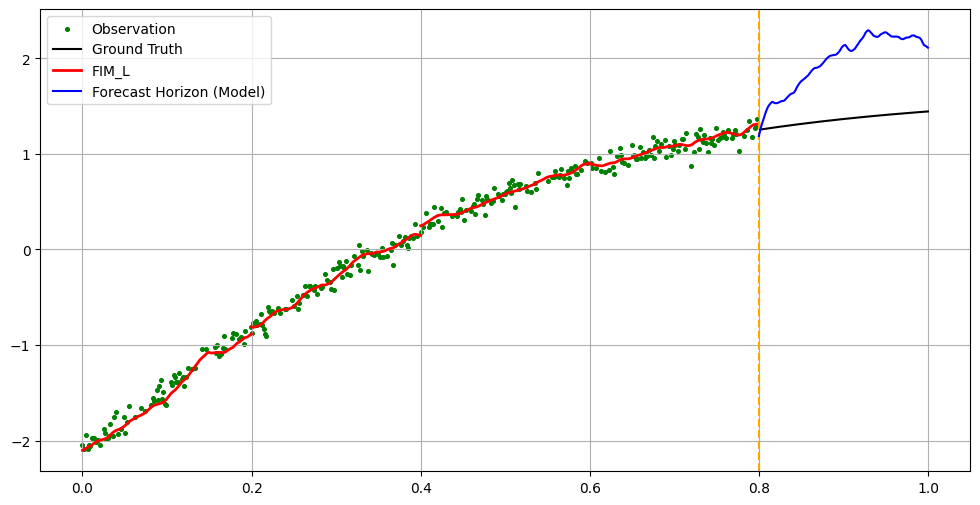
\includegraphics[width=\linewidth]{assets/test1.png}
    \caption{Example on the live dataset with $\text{horizon}=128$, using the PE + CSL model version.
    }\label{fig:test1}
\end{figure}
\begin{figure}[h!]
    \centering
    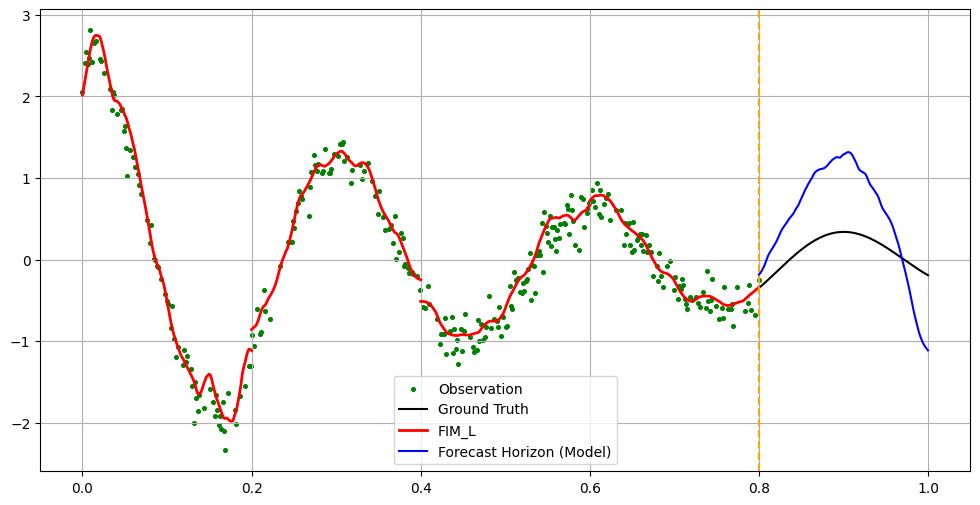
\includegraphics[width=\linewidth]{assets/test2.png}
    \caption{Example on the live dataset with $\text{horizon}=128$, using the PE + CSL model version.
    }\label{fig:test2}
\end{figure}
\begin{figure}[h!]
    \centering
    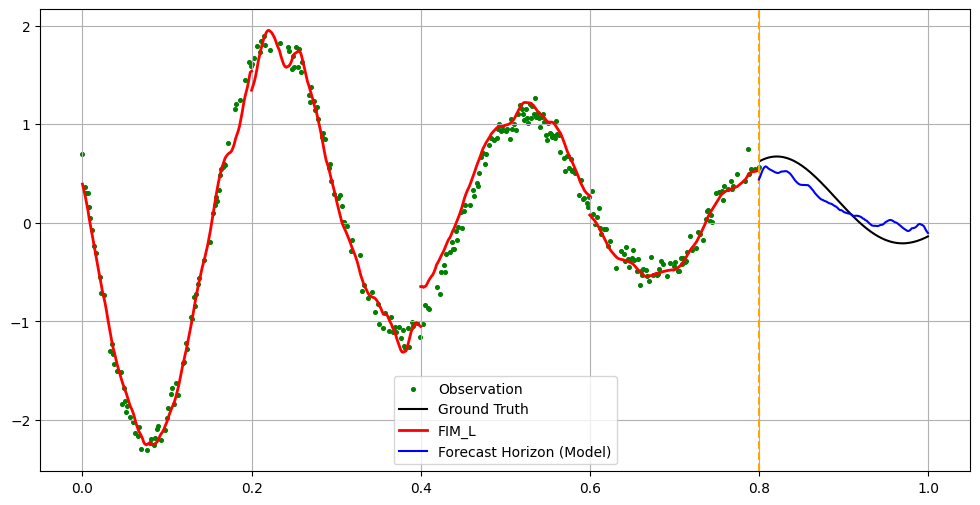
\includegraphics[width=\linewidth]{assets/test3.png}
    \caption{Example on the live dataset with $\text{horizon}=128$, using the PE + CSL model version.
    }\label{fig:test3}
\end{figure}
\begin{figure}[h!]
    \centering
    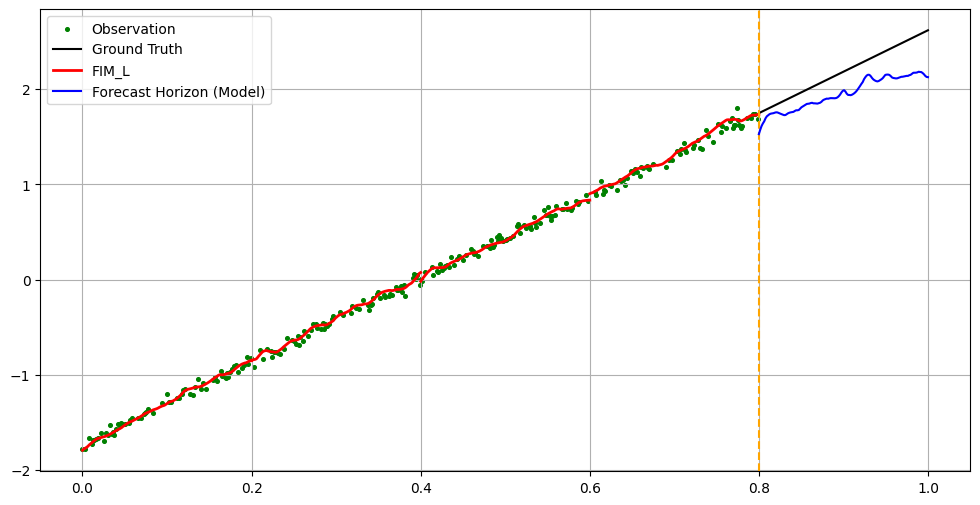
\includegraphics[width=\linewidth]{assets/test4.png}
    \caption{Example on the live dataset with $\text{horizon}=128$, using the PE + CSL model version.
    }\label{fig:test4}
\end{figure}
\begin{figure}[h!]
    \centering
    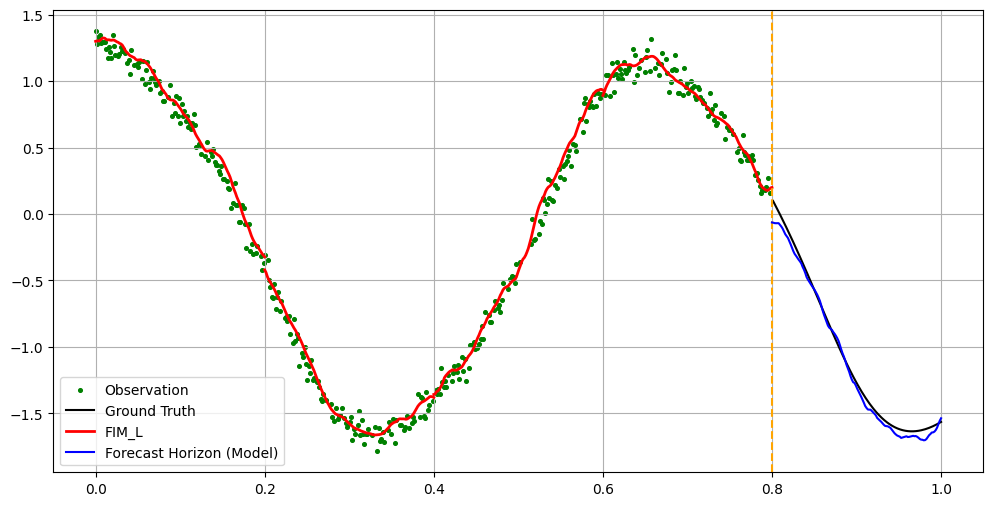
\includegraphics[width=\linewidth]{assets/test5.png}
    \caption{Example on the live dataset with $\text{horizon}=128$, using the PE + CSL model version.
    }\label{fig:test5}
\end{figure}
\end{document}

% This document was modified from the file originally made available by
% Pat Langley and Andrea Danyluk for ICML-2K. This version was created
% by Iain Murray in 2018, and modified by Alexandre Bouchard in
% 2019 and 2021 and by Csaba Szepesvari, Gang Niu and Sivan Sabato in 2022.
% Modified again in 2023 and 2024 by Sivan Sabato and Jonathan Scarlett.
% Previous contributors include Dan Roy, Lise Getoor and Tobias
% Scheffer, which was slightly modified from the 2010 version by
% Thorsten Joachims & Johannes Fuernkranz, slightly modified from the
% 2009 version by Kiri Wagstaff and Sam Roweis's 2008 version, which is
% slightly modified from Prasad Tadepalli's 2007 version which is a
% lightly changed version of the previous year's version by Andrew
% Moore, which was in turn edited from those of Kristian Kersting and
% Codrina Lauth. Alex Smola contributed to the algorithmic style files.
